\section{Study 3 --- Financial Viability}
\label{sec:method-study3}

Sovereignty has to be paid for. The first two studies asked whether a provider is
legally able to protect the data it holds and technically able to run the work,
but both of those are things a provider must keep buying. Data centres, servers
and network capacity are not bought once, and a provider that cannot fund them
cannot offer the services counted in \cref{sec:method-study2}, whatever its legal
standing. A provider that runs out of money altogether offers nothing at all.

The economics make this harder for a European entrant than for the incumbent.
The \ac{OECD} finds that establishing a cloud service carries high fixed costs,
and that most of the capital involved --- data centres, network infrastructure,
servers and hardware --- is sunk, in the sense that it cannot be recovered if the
provider withdraws \cite{OECD_CloudCompetition_2025}. Committing to build is
therefore close to irreversible. Scale then compounds the difficulty: because the
largest providers can invest at a level almost no entrant can match, they operate
at lower marginal cost, and the same report concludes that a supplier unwilling
to match those investment levels \enquote{will likely incur higher costs to
deliver the same level of service as the hyperscalers}
\cite{OECD_CloudCompetition_2025}.

That is the position every provider in this study occupies, and it carries a
consequence for sovereignty that the first two studies cannot see. A sovereign
alternative exists in practice only if somebody can afford to build and keep
running it. A provider may hold the strongest legal position in Europe and still
be unable to fund the next data centre, in which case the sovereignty it offers
is available only for the workloads it already supports.

This study therefore examines the money behind each provider, and what it implies
for the years a contract has to run: how fast each is closing the capability gap
against the \acs{AWS} baseline and when it would draw level, what it earns, what
it spends to gain that ground, and where that money comes from. The aim is to
establish how far finance accounts for the progress these providers have made,
and for the distance still left.

Five providers are carried into this study, with \acs{AWS} again as the baseline.
\Cref{tab:study3-providers} gives them, and what the first two studies found
about each.

\begin{table}[htbp]
  \centering
  \caption{The five providers carried into Study~3, with their results from the
           first two studies.}
  \label{tab:study3-providers}
  \small
  \begin{tabularx}{\textwidth}{@{}l l r r X@{}}
    \toprule
    \textbf{Provider} & \textbf{Parent company}
      & \textbf{Sov.} & \textbf{Cap.}
      & \textbf{Reason for inclusion} \\
    \midrule
    \acs{AWS}      & Amazon.com, Inc.      & ---  & 100 & Baseline \\
    \midrule
    T-Cloud Public & Deutsche Telekom \acs{AG} & 66.2 & 72 & Highest capability \\
    OVHcloud       & OVH Groupe            & 58.8 & 56 & Second highest capability \\
    STACKIT        & Schwarz Group         & 82.5 & 44 & Third highest capability \\
    Scaleway       & iliad Group           & 72.5 & 40 & Fourth highest capability \\
    IONOS          & United Internet \acs{AG} & 52.5 & 27 & Finances publicly accessible \\
    \bottomrule
  \end{tabularx}
\end{table}

Four of the five are the highest-ranked on capability in
\cref{sec:method-study2}. IONOS was included because it publishes financial
accounts of its own, which is what this study needs. 

Sovereignty rank played no part in the selection, and the table shows why it
could not have: only STACKIT clears every minimum in \cref{sec:method-study1}.
Carrying forward only the providers that passed would have left a single
candidate and nothing to compare it against. This study aims to evaluate whether
the financial position of the providers is consistent with the sovereignty and
capability they offer. 


\subsection{Closing the gap to AWS}

Will these \acs{EU} cloud providers catch up with hyperscalers like \acs{AWS}?
Two figures are used to answer that: the \textbf{parity speed}, the rate of
growth in capability each provider has achieved since it launched, and the
\textbf{parity year}, the year it would reach the same capability as \acs{AWS} if
that growth continues.

Both rest on a starting year, and the providers do not share one. To establish
it, the development phase of each was examined, as shown in
\cref{fig:launch-dates}, and the external launch date was considered --- the year the platform was made available to the general public, not to internal teams or a free trial.

\begin{figure}[htbp]
  \centering
  % Years are plotted as an offset from 1999: using the year itself as a
  % coordinate multiplies out past TikZ's maximum dimension.
  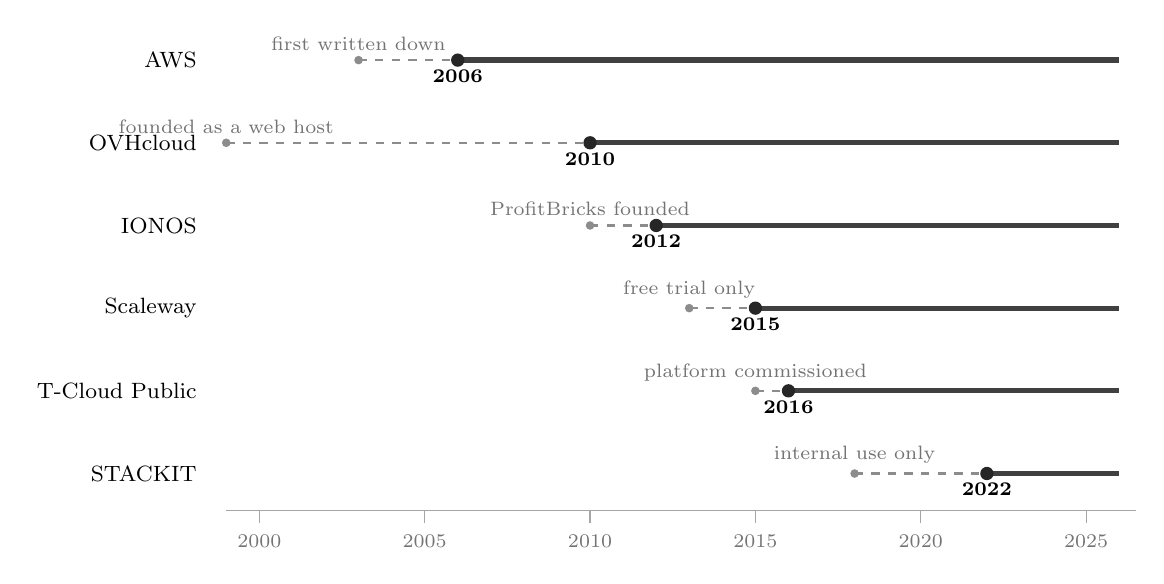
\begin{tikzpicture}[x=0.42cm, y=1.05cm]
    \def\yzero{1999}
    \draw[black!35] (0,-0.45) -- (27.5,-0.45);
    \foreach \yr in {2000,2005,2010,2015,2020,2025} {
      \pgfmathsetmacro\xx{\yr-\yzero}
      \draw[black!35] (\xx,-0.45) -- (\xx,-0.60);
      \node[below, font=\scriptsize, black!55] at (\xx,-0.62) {\yr};
    }
    \foreach \row/\start/\launch/\name/\origin in {%
      5/2003/2006/{\acs{AWS}}/{first written down},
      4/1999/2010/{OVHcloud}/{founded as a web host},
      3/2010/2012/{IONOS}/{ProfitBricks founded},
      2/2013/2015/{Scaleway}/{free trial only},
      1/2015/2016/{T-Cloud Public}/{platform commissioned},
      0/2018/2022/{STACKIT}/{internal use only}}
    {
      \pgfmathsetmacro\xs{\start-\yzero}
      \pgfmathsetmacro\xl{\launch-\yzero}
      \node[left, font=\footnotesize] at (-0.6,\row) {\name};
      \draw[black!45, dashed, line width=0.9pt] (\xs,\row) -- (\xl,\row);
      \node[circle, fill=black!45, inner sep=1.1pt] at (\xs,\row) {};
      \node[above, font=\scriptsize, black!55] at (\xs,\row) {\origin};
      \draw[black!75, line width=1.9pt] (\xl,\row) -- (27,\row);
      \node[circle, fill=black!85, inner sep=1.7pt] at (\xl,\row) {};
      \node[below, font=\scriptsize\bfseries] at (\xl,\row) {\launch};
    }
  \end{tikzpicture}
  \caption{Launch phase of each provider — the time taken from the beginning of development until the service is made publicly available.}
  \label{fig:launch-dates}
\end{figure}

The dashed part is the time spent building before anything could be bought; the solid part is the time
on sale. The external launch year used in the calculation is shown in
bold. 

\begin{itemize}
  \item \textbf{\acs{AWS}} --- the idea was written down inside Amazon in 2003
        and built from 2004 \cite{Black_EC2Origins_2009}. Its storage service
        went on sale in \textbf{2006}, the year used
        \cite{AWS_FirstFiveYears}.
  \item \textbf{OVHcloud} --- founded in 1999, but as a web hosting company. It
        began building its own data centres in 2006 and sold no cloud product
        until \textbf{2010}, the year used \cite{OVHcloud_History}.
  \item \textbf{IONOS} --- the platform is ProfitBricks, founded in Berlin in
        2010 \cite{IONOS_ProfitBricks_2018} and selling by \textbf{2012}, the
        year used: it had around a thousand customers by that November
        \cite{ProfitBricks_DCK_2012}. United Internet bought it in 2017 and the
        business was renamed IONOS in 2018
        \cite{IONOS_ProfitBricks_2018}, so the familiar name is six years
        younger than the platform behind it.
  \item \textbf{Scaleway} --- ran from 2013 as a free trial under the name
        Online Labs. It went on sale as Scaleway in \textbf{2015}, the year
        used \cite{Scaleway_About}.
  \item \textbf{T-Cloud Public} --- the platform was commissioned in 2015 under
        a partnership with Huawei and opened to customers as Open Telekom Cloud
        in \textbf{2016}, the year used \cite{OTC_GoesLive_2016}.
  \item \textbf{STACKIT} --- built in 2018 to run Lidl and Kaufland alone. It
        opened to customers outside the Schwarz group in \textbf{2022}, the year
        used \cite{STACKIT_Launch_2022}.
\end{itemize}

The dashed part is therefore left out in every case, the baseline included.
\acs{AWS} ran three years before it had anything to sell, and STACKIT four;
neither is credited with them.

With a start year fixed, the capability score becomes a rate. The parity speed is
the score divided by the years the provider has been selling, and the parity year
is the point at which that speed would carry it to the baseline of 100. The year
of assessment is 2026 throughout.

\begin{align}
  \label{eq:parity-speed}
  \text{parity speed (points/year)}
    &= \frac{\text{score}}{2026 - \text{launch year}} \\[0.6em]
  \label{eq:parity-year}
  \text{parity year}
    &\approx 2026 + \frac{100 - \text{score}}{\text{parity speed}}
\end{align}

Worked through for T-Cloud Public: it scores 72.1 and has been selling since
2016, so ten years for 72.1 points, a rate of 7.2 points a year. The remaining
27.9 points at that rate take a further four years, giving 2030.

The parity year is an illustration, not a forecast, for three reasons. First, no
provider has undertaken to keep improving at the rate it has managed so far, and
none is obliged to. Second, it assumes progress is even, which it is not: the first
services a provider builds are the ones its customers ask for most, and the
remainder get harder.

Third, it holds the baseline still. \acs{AWS} sits at 100 throughout, but it is not
a fixed target. It adds services continuously, and the catalogue used in
\cref{sec:method-study2} records only what it offered at the time of assessment.
A provider closing on 100 is therefore closing on where \acs{AWS} stood in 2026,
not where it will stand in 2038, for example. Every date that follows is the earliest a
provider could arrive, on the most favourable reading available to it, and the
real distance is wider than the chart can show. Whether it is wider by a few
years or by an unbridgeable margin depends on how fast \acs{AWS} keeps extending
its own catalogue, which this study does not attempt to predict.

The figure is reported because it expresses the gap in years rather than points,
and years are the unit a contract is written in.

\Cref{fig:parity-projection} draws the result. The solid lines are the record so
far, from launch to the year of assessment. The dashed lines carry each rate
forward to the baseline.

\begin{figure}[htbp]
  \centering
  \begin{tikzpicture}
    \begin{axis}[
      width=0.96\textwidth, height=8.2cm,
      xmin=2006, xmax=2066, ymin=0, ymax=108,
      xlabel={Year}, ylabel={Capability score},
      xlabel style={font=\footnotesize}, ylabel style={font=\footnotesize},
      xtick={2006,2016,2026,2036,2046,2056,2066},
      ytick={0,20,40,60,80,100},
      ticklabel style={font=\footnotesize},
      % years are years, not quantities: suppress the thousands separator
      scaled x ticks=false,
      x tick label style={/pgf/number format/1000 sep={}},
      grid=major, grid style={black!10},
      axis on top,
      legend style={at={(0.5,-0.22)}, anchor=north, legend columns=3,
                    font=\footnotesize, draw=none, column sep=1ex},
      tick style={draw=none},
      axis x line*=bottom, axis y line*=left,
      clip=false,
    ]
      % projection zone, everything right of the year of assessment
      \fill[black!4] (axis cs:2026,0) rectangle (axis cs:2066,108);
      % the baseline the providers are measured against
      \addplot[cBase, dashed, very thick, mark=none, forget plot]
        coordinates {(2006,100) (2066,100)};
      \node[anchor=south east, font=\scriptsize, cBase]
        at (axis cs:2066,100) {\acs{AWS} baseline};
      % year of assessment, and the Digital Decade target
      \draw[black!45, dashed] (axis cs:2026,0) -- (axis cs:2026,108);
      \node[anchor=south, font=\scriptsize, black!55, rotate=90]
        at (axis cs:2025.2,2) {assessed 2026};
      \draw[black!45, dashed] (axis cs:2030,0) -- (axis cs:2030,108);
      \node[anchor=south, font=\scriptsize, black!55, rotate=90]
        at (axis cs:2029.2,2) {2030 EC Digital Decade};

      % record so far (solid) and the rate carried forward (dashed)
      \addplot[cProvA, very thick] coordinates {(2016,0) (2026,72.1)};
      \addplot[cProvA, thick, dashed, mark=*, mark size=1.6pt,
               forget plot] coordinates {(2026,72.1) (2029.9,100)};
      \addplot[cProvC, very thick] coordinates {(2022,0) (2026,44.1)};
      \addplot[cProvC, thick, dashed, mark=*, mark size=1.6pt,
               forget plot] coordinates {(2026,44.1) (2031.1,100)};
      \addplot[cProvB, very thick] coordinates {(2010,0) (2026,56.2)};
      \addplot[cProvB, thick, dashed, mark=*, mark size=1.6pt,
               forget plot] coordinates {(2026,56.2) (2038.5,100)};
      \addplot[cProvD, very thick] coordinates {(2015,0) (2026,40.3)};
      \addplot[cProvD, thick, dashed, mark=*, mark size=1.6pt,
               forget plot] coordinates {(2026,40.3) (2042.3,100)};
      \addplot[cProvE, very thick] coordinates {(2012,0) (2026,26.8)};
      \addplot[cProvE, thick, dashed, mark=*, mark size=1.6pt,
               forget plot] coordinates {(2026,26.8) (2064.2,100)};
      \legend{T-Cloud Public, STACKIT, OVHcloud, Scaleway, IONOS}
    \end{axis}
  \end{tikzpicture}
  \caption{Capability added since launch (solid) and the same rate carried
           forward to the \acs{AWS} baseline (dashed). The shaded area is
           projection rather than record.}
  \label{fig:parity-projection}
\end{figure}

The steepest line belongs to the youngest provider. STACKIT has been selling for
four years and has added capability faster than anyone in the set, which is what
places it at the baseline in 2031 despite starting last. T-Cloud Public arrives a
year earlier from a higher score and a gentler slope. Both fall close to the
Union's 2030 target for digital capability, and the remaining three do not:
OVHcloud in 2038, Scaleway in 2042, and IONOS not until the 2060s.

The IONOS figure indicates a direction rather than a date. Thirty-eight years is
past any horizon a procurement decision occupies, and the figure reflects what
IONOS is: a business whose capability score is low because it sells hosting and
domains rather than infrastructure, not because it is building infrastructure
slowly. The projection assumes every provider is running the same race, and that
is the assumption it exposes.

\subsection{Cloud Providers, and their parent company}

The parity speed shows how fast each provider has been adding capability, but not
what that capability cost or who paid for it. Those are the questions the rest of
this study addresses, and it addresses them by assessing each provider together
with the company that owns it rather than on its own.

\Cref{tab:study3-providers} shows why. Every provider sits inside a parent
company, the baseline included --- Amazon reports
\acs{AWS}'s results separately within its own accounts. A provider with an owner
behind it can be funded
through years of losses, can build at a scale its own revenue would never
support, and can be sustained for strategic reasons that have nothing to do with
whether the cloud business itself is profitable.

The parents are not alike, and the difference matters more than the fact of
having one. Deutsche Telekom, Schwarz, iliad and Amazon all run substantial
businesses outside cloud. Deutsche Telekom and iliad are telecommunications
operators; Schwarz and Amazon are retailers. From any of them a cloud arm can
be subsidised indefinitely. OVH Groupe does not:
it is the listed holding company for the cloud business and essentially nothing
else, majority-held by the founding family. When OVHcloud needs capital it goes
to the markets, which is what it did in 2021 \cite{OVHcloud_IPO}. When STACKIT
needs capital it asks Schwarz \cite{SchwarzDigits_Luebbenau_2025}.


The owners also differ in how much they are willing to say, and that turns out to
shape what this study can measure. \Cref{tab:study3-disclosure} sets out what each
one actually publishes.

\begin{table}[htbp]
  \centering
  \caption{What each owner publishes about its cloud business.}
  \label{tab:study3-disclosure}
  \footnotesize
  \begin{tabularx}{\textwidth}{@{}l l X l@{}}
    \toprule
    Provider & Owner & Revenue of the cloud business & Revenue by country \\
    \midrule
    \acs{AWS}      & Amazon           & Published, as one of three reporting segments & Not published \\
    OVHcloud       & OVH Groupe       & Published --- it is the whole company          & Published, three regions \\
    IONOS          & United Internet  & Published separately since 2020                & German and non-German only \\
    T-Cloud Public & Deutsche Telekom & Not published                                  & Published, as percentages \\
    Scaleway       & iliad            & Not published                                  & Published, country by country \\
    STACKIT        & Schwarz Group    & Not published                                  & Not published \\
    \bottomrule
  \end{tabularx}

  \vspace{2pt}
  \footnotesize
  Sources. \cite{Amazon_10K_2025,OVHcloud_URD_2025,IONOS_AR_2025,UnitedInternet_AR_2025,%
  DT_AR_2025,Iliad_AFR_2025,Schwarz_Figures_FY2025}.
\end{table}

The pattern follows how each owner is held. Amazon, OVH Groupe, United Internet
and IONOS are listed and publish the most. Deutsche Telekom is listed and iliad
was until 2021, and both publish where their revenue is earned but not what their
cloud business takes in. The Schwarz Group is privately held, answers to no
stock-market regulator on the point, and publishes one worldwide turnover figure a
year and nothing more \cite{Schwarz_Figures_FY2025}.


\subsection{Investments and commitments}
\label{sec:study3-investment}

Building the tools and services that customers' use cases require costs a great
deal in resources --- data centres, hardware, and the staff to run both --- and
none of that appears in a rate of improvement. This section therefore establishes
how much capital stands behind each provider, where that capital came from, and on
what timetable it was committed.

\Cref{fig:investment-timeline} presents that capital in full. Each row is a
provider and each circle a single commitment, positioned at the year it was
announced, with circle area proportional to the amount. A dashed, open circle marks
a commitment announced without a figure: a sum was committed, but its size was
never disclosed, so no area can represent it.

\begin{figure}[htbp]
  \centering
  \begin{tikzpicture}
    \begin{axis}[
      width=0.95\textwidth, height=7.4cm,
      xmin=2014.3, xmax=2026.9,
      xtick={2015,2016,2017,2018,2019,2020,2021,2022,2023,2024,2025,2026},
      xticklabel style={font=\scriptsize, rotate=45, anchor=north east,
                        /pgf/number format/1000 sep={}},
      ymin=0.4, ymax=6.6,
      ytick={1,2,3,4,5,6},
      yticklabels={STACKIT,Scaleway,{T-Cloud Public},IONOS,OVHcloud,{\acs{AWS} in Europe}},
      yticklabel style={font=\scriptsize},
      xmajorgrids=true, ymajorgrids=true, grid style={gray!20},
      axis lines*=left,
      clip=false,
    ]
      \draw[draw=black!45, line width=0.6pt] (axis cs:2024.00,6) circle[radius=15.25pt];
      \draw[draw=black!45, line width=0.6pt] (axis cs:2025.30,2) circle[radius=2.45pt];
      \draw[draw=black!45, line width=0.6pt] (axis cs:2024.00,4) circle[radius=2.41pt];
      \draw[draw=black!45, line width=0.6pt] (axis cs:2026.00,3) circle[radius=1.96pt];
      \draw[draw=black!40, line width=0.5pt, dash pattern=on 1.4pt off 1.2pt] (axis cs:2026.00,5) circle[radius=2.30pt];
      \draw[draw=black!40, line width=0.5pt, dash pattern=on 1.4pt off 1.2pt] (axis cs:2026.00,2) circle[radius=2.30pt];
      \draw[draw=black!40, line width=0.5pt, dash pattern=on 1.4pt off 1.2pt] (axis cs:2026.40,1) circle[radius=2.30pt];
      \draw[fill=black!35, draw=black!45, line width=0.3pt] (axis cs:2018.00,4) circle[radius=1.50pt];
      \draw[fill=black!35, draw=black!45, line width=0.3pt] (axis cs:2016.20,3) circle[radius=1.50pt];
      \draw[fill=black!35, draw=black!45, line width=0.3pt] (axis cs:2015.00,2) circle[radius=1.50pt];
      \draw[fill=black!35, draw=black!45, line width=0.3pt] (axis cs:2022.00,1) circle[radius=1.50pt];
      \draw[fill=cBase, fill opacity=0.75, draw=cBase!65!black, line width=0.4pt] (axis cs:2026.00,6) circle[radius=8.11pt];
      \draw[fill=cBase, fill opacity=0.75, draw=cBase!65!black, line width=0.4pt] (axis cs:2023.62,6) circle[radius=7.66pt];
      \draw[fill=cProvE, fill opacity=0.75, draw=cProvE!65!black, line width=0.4pt] (axis cs:2025.00,1) circle[radius=6.64pt];
      \draw[fill=cBase, fill opacity=0.75, draw=cBase!65!black, line width=0.4pt] (axis cs:2024.00,6) circle[radius=6.09pt];
      \draw[fill=cBase, fill opacity=0.75, draw=cBase!65!black, line width=0.4pt] (axis cs:2023.00,6) circle[radius=5.82pt];
      \draw[fill=cProvE, fill opacity=0.75, draw=cProvE!65!black, line width=0.4pt] (axis cs:2025.90,1) circle[radius=5.14pt];
      \draw[fill=cProvA, fill opacity=0.75, draw=cProvA!65!black, line width=0.4pt] (axis cs:2024.85,2) circle[radius=4.14pt];
      \draw[fill=cBase, fill opacity=0.75, draw=cBase!65!black, line width=0.4pt] (axis cs:2022.00,6) circle[radius=3.64pt];
      \draw[fill=cBase, fill opacity=0.75, draw=cBase!65!black, line width=0.4pt] (axis cs:2024.38,6) circle[radius=3.13pt];
      \draw[fill=cProvB, fill opacity=0.75, draw=cProvB!65!black, line width=0.4pt] (axis cs:2025.00,5) circle[radius=3.10pt];
      \draw[fill=cProvC, fill opacity=0.75, draw=cProvC!65!black, line width=0.4pt] (axis cs:2025.00,3) circle[radius=2.98pt];
      \draw[fill=cProvD, fill opacity=0.75, draw=cProvD!65!black, line width=0.4pt] (axis cs:2022.72,4) circle[radius=2.81pt];
      \draw[fill=cProvE, fill opacity=0.75, draw=cProvE!65!black, line width=0.4pt] (axis cs:2021.00,1) circle[radius=2.62pt];
      \draw[fill=cProvB, fill opacity=0.75, draw=cProvB!65!black, line width=0.4pt] (axis cs:2021.00,5) circle[radius=2.46pt];
      \draw[fill=cProvD, fill opacity=0.75, draw=cProvD!65!black, line width=0.4pt] (axis cs:2017.00,4) circle[radius=2.46pt];
      \draw[fill=cProvD, fill opacity=0.75, draw=cProvD!65!black, line width=0.4pt] (axis cs:2023.00,4) circle[radius=2.46pt];
      \draw[fill=cProvB, fill opacity=0.75, draw=cProvB!65!black, line width=0.4pt] (axis cs:2017.00,5) circle[radius=2.40pt];
      \draw[fill=cProvB, fill opacity=0.75, draw=cProvB!65!black, line width=0.4pt] (axis cs:2015.00,5) circle[radius=2.22pt];
      \draw[fill=cProvB, fill opacity=0.75, draw=cProvB!65!black, line width=0.4pt] (axis cs:2016.00,5) circle[radius=2.19pt];
      \draw[fill=cProvC, fill opacity=0.75, draw=cProvC!65!black, line width=0.4pt] (axis cs:2024.00,3) circle[radius=2.16pt];
      \draw[fill=cProvC, fill opacity=0.75, draw=cProvC!65!black, line width=0.4pt] (axis cs:2022.85,3) circle[radius=2.12pt];
      \draw[fill=cProvB, fill opacity=0.75, draw=cProvB!65!black, line width=0.4pt] (axis cs:2022.00,5) circle[radius=2.11pt];
      \draw[fill=cProvA, fill opacity=0.75, draw=cProvA!65!black, line width=0.4pt] (axis cs:2023.00,2) circle[radius=2.01pt];
      \draw[fill=cProvC, fill opacity=0.75, draw=cProvC!65!black, line width=0.4pt] (axis cs:2015.85,3) circle[radius=1.90pt];
      \draw[fill=cProvD, fill opacity=0.75, draw=cProvD!65!black, line width=0.4pt] (axis cs:2023.28,4) circle[radius=1.61pt];
      \draw[fill=cProvC!8, draw=cProvC!70!black, line width=0.6pt, dash pattern=on 1.6pt off 1.2pt] (axis cs:2021.00,3) circle[radius=2.30pt];
      \draw[fill=cProvC!8, draw=cProvC!70!black, line width=0.6pt, dash pattern=on 1.6pt off 1.2pt] (axis cs:2023.20,3) circle[radius=2.30pt];
    \end{axis}
  \end{tikzpicture}

  \vspace{4pt}
  {\footnotesize\raggedright
  \tikz[baseline=-0.55ex]\draw[fill=black!55, fill opacity=0.75, draw=black!70,
    line width=0.4pt] (0,0) circle[radius=2.6pt];~counted as capital \quad
  \tikz[baseline=-0.55ex]\draw[fill=black!8, draw=black!65, line width=0.6pt,
    dash pattern=on 1.6pt off 1.2pt] (0,0) circle[radius=2.3pt];~amount not published \quad
  \tikz[baseline=-0.55ex]\draw[draw=black!45, line width=0.6pt]
    (0,0) circle[radius=2.6pt];~not capital, counted nowhere \quad
  \tikz[baseline=-0.55ex]\draw[fill=black!35, draw=black!45, line width=0.3pt]
    (0,0) circle[radius=1.5pt];~launch,\par
  \vspace{3pt}
  Circle area is proportional to the amount; colour identifies the provider.
  \Cref{tab:study3-milestones} lists every circle shown.\par}
  \caption{Capital commitments year by year, 2015--2026.}
  \label{fig:investment-timeline}
\end{figure}

\Cref{tab:study3-milestones} lists every circle on the chart.

\begin{table}[htbp]
  \centering
  \caption{Every capital commitment on the timeline, 2015--2026, in millions of euros.}
  \label{tab:study3-milestones}
  \footnotesize
  \setlength{\tabcolsep}{4pt}
  \begin{tabularx}{\textwidth}{@{}l X l r l@{}}
    \toprule
    Year & What & From & Amount & Notes \\
    \midrule
    \multicolumn{5}{@{}l}{\textit{\acs{AWS} in Europe}} \\
    2022 & \acs{AWS} Europe (Milan) Region            & Amazon & 2\,000  &  \\
    2023 & European Sovereign Cloud, Brandenburg      & Amazon & 7\,800  & To 2040 \\
    2024 & \acs{AWS} Europe (Frankfurt) Region        & Amazon & 8\,800  & 2024--2026 \\
    2024 & \acs{AWS} Europe (Spain) Region, Arag\'on  & Amazon & 15\,700 & Over a decade \\
    2024 & Milan Region expansion                     & Amazon & 1\,200  & Five years \\
    2024 & Amazon capital spending, all businesses    & Amazon & 76\,682 &  one year worldwide \\
    2026 & Spain increase                             & Amazon & 18\,000 & To 2035 \\
    \midrule
    \multicolumn{5}{@{}l}{\textit{OVHcloud}} \\
    2015 & First syndicated debt                      & Debt   &    267  &  \\
    2016 & KKR and TowerBrook stake                   & Equity &    250  &  \\
    2017 & Syndicated loan                            & Debt   &    400  &  \\
    2021 & Euronext Paris listing                     & Equity &    450  &  \\
    2022 & \acs{EIB} green loan                       & Debt   &    200  &  \\
    2025 & High-yield bond and green loan             & Debt   & 1\,150  &  \\
    2026 & \acs{EC} framework contract                &        &         &  contract won \\
    \midrule
    \multicolumn{5}{@{}l}{\textit{IONOS}} \\
    2017 & Warburg Pincus, 33.3\,\% of the business   & Equity &    450  &  \\
    2018 & Cloud portfolio launch                     &        &         &  \\
    2023 & Frankfurt listing                          & Equity &    447  &  \\
    2023 & Syndicated loan                            & Debt   &    800  &  \\
    2023 & \acs{IPCEI}-CIS, granted portion           & \acs{EU} &   17  &  \\
    2024 & ITZBund framework                          &        &    410  &  ceiling on revenue \\
    \midrule
    \multicolumn{5}{@{}l}{\textit{T-Cloud Public}} \\
    2016 & Service launch                             &        &         &  \\
    2016 & Biere phase 2 syndicated loan              & Debt   &    100  &  \\
    2021 & Amsterdam twin data centre                 & Deutsche Telekom & & Undisclosed figure \\
    2023 & Systems Solutions cash capex               & Deutsche Telekom & 210 & Reported spending \\
    2023 & \acs{IPCEI}-CIS participation              & \acs{EU} &  & Undisclosed figure \\
    2024 & Systems Solutions cash capex               & Deutsche Telekom & 229 & Reported spending \\
    2025 & Industrial \acs{AI} Cloud Munich, with NVIDIA & Deutsche Telekom & 1\,000 &  \\
    2026 & Federal \acs{AI} cloud                     &        &    125  &  contract won \\
    \midrule
    \multicolumn{5}{@{}l}{\textit{Scaleway}} \\
    2015 & Rebranded to Scaleway                      &        &         &  \\
    2023 & \acs{IPCEI}-CIS grant                      & \acs{EU} &  150  &  \\
    2025 & iliad \acs{AI} commitment                  & iliad  & 3\,000  &  \\
    2025 & OpCore stake sold                          &        &    440  &  proceeds of a sale \\
    2026 & \acs{EC} framework contract                &        &         &  contract won \\
    \midrule
    \multicolumn{5}{@{}l}{\textit{STACKIT}} \\
    2021 & XM~Cyber acquisition                       & Schwarz &   592  &  \\
    2022 & Commercial launch                          &        &         &  \\
    2025 & L\"ubbenau data centre                     & Schwarz & 11\,000 & Phase 1 by 2027 \\
    2026 & Dummerstorf data centre                    & Schwarz & 5\,600  & To 2033 \\
    2026 & \acs{EC} framework contract                &        &         &  contract won \\
    \bottomrule
  \end{tabularx}

  \vspace{4pt}
  {\footnotesize\raggedright
  Sources. \cite{AWS_SovereignCloud_Investment_2024,AWS_Frankfurt_Investment_2024,%
  Amazon_Spain_Investment_2026,OVHcloud_IPO,OVHcloud_RegDoc_2021,OVHcloud_URD_2025,%
  IONOS_AR_2025,UnitedInternet_AR_2025,IPCEI_CIS_2023,DT_AR_2025,%
  Iliad_AIInvestment_2025,Schwarz_XMCyber_2021,SchwarzDigits_Luebbenau_2025,%
  SchwarzDigits_Dummerstorf_2026}.\par}
\end{table}

Few of these announcements say when the money will be spent. Only seven of them
give a completion date or a duration, and all seven come from two owners: five
from Amazon and two from the Schwarz Group. OVHcloud, IONOS, Deutsche Telekom and
iliad attached no timetable to any of their commitments. Only two figures in the
whole table, both from Deutsche Telekom, record money that was actually spent,
because they come from an annual report rather than from an announcement. No
provider publishes what it has built against what it announced, so the table
records intentions and money raised, not construction.

Three of the counted figures are also less precise than they appear:

\begin{enumerate}
  \item \textbf{Deutsche Telekom's capital spending overstates the cloud
  investment.} The figures for 2023 and 2024 cover the whole Systems Solutions
  segment, of which Open Telekom Cloud is only one part. Deutsche Telekom
  publishes no figure for the cloud service alone, so the amount actually spent
  on it is smaller than the 439 million euros shown \cite{DT_AR_2025}.

  \item \textbf{Only part of iliad's 3 billion euros is for Scaleway.} The
  commitment is shared between Scaleway, the data-centre company OpCore and the
  Kyutai research laboratory, and iliad did not say how it is divided or by when
  it will be spent \cite{Iliad_AIInvestment_2025}. Scaleway's own share is
  therefore unknown.

  \item \textbf{STACKIT's only counted spending before 2025 was not on cloud
  infrastructure.} The 592 million euros is the Schwarz Group's purchase of the
  security software company XM~Cyber for 700 million US dollars in 2021
  \cite{Schwarz_XMCyber_2021}. It is counted because it was part of Schwarz's
  digital build-out, but it means that no Schwarz spending on STACKIT's
  infrastructure itself was disclosed before the L\"ubbenau announcement.
\end{enumerate}

The timeline reveals four features of how these providers have been funded:

\begin{enumerate}
  \item \textbf{The providers raised their money in two different patterns.}
  OVHcloud and IONOS each show a series of moderate amounts spread over ten years:
  six for OVHcloud and four for IONOS, the largest being OVHcloud's 1.15 billion
  euros in 2025. T-Cloud Public follows a similar pattern, with four amounts
  between 100 million and 1 billion euros. STACKIT and Scaleway show the opposite:
  almost no announced investment for several years, followed by one or two very
  large commitments at the end of the period. The difference reflects where the
  money came from, which is discussed in the next part of this section.

  \item \textbf{The largest commitments are all recent.} No commitment of 3 billion
  euros or more was announced before 2023. As \Cref{tab:study3-milestones} shows,
  none of the largest \acs{EU} commitments has yet reached the completion date set
  in its own announcement: they run to 2027 or 2033, or give no date at all.

  \item \textbf{Deutsche Telekom has left two commitments unquantified.} It is the
  only owner to have announced capital commitments without stating their size:
  the Amsterdam twin data centre in 2021 and its participation in the
  \acs{IPCEI}-CIS programme in 2023. Neither can therefore be included in any
  total.

  \item \textbf{AWS follows the same pattern as STACKIT, but earlier and on a
  larger scale.} Its row also consists of a few very large commitments rather than
  many smaller ones. In both cases the money comes from a parent company whose
  resources far exceed those of the cloud business itself: Amazon for \acs{AWS},
  and the Schwarz Group for STACKIT.
\end{enumerate}

\subsubsection*{Scope of what is counted as capital}

Eleven of the circles in \Cref{fig:investment-timeline} are drawn in grey and are
not counted in any total in this study. Four of them are product launches, which
carry no amount. The remaining seven fall into four categories:

\begin{enumerate}
  \item \textbf{Contracts won.} A contract is money a provider expects to earn,
  not money it has invested. When the German Federal IT Centre awarded IONOS a
  five-year framework contract in April 2024, the widely reported figure of 410
  million euros was a ceiling with no guarantee of orders, and IONOS itself
  expected revenue in the low hundreds of millions \cite{IONOS_ITZBund_2024}.
  T-Systems' share of the German federal \acs{AI} cloud contract is the same kind
  of figure.

  \item \textbf{Sale of an asset.} When iliad sold half of its data-centre
  subsidiary OpCore to InfraVia in 2025, the 440 million euros it received was
  income from a sale, not an investment \cite{Iliad_Results_FY2025}.

  \item \textbf{Contracts with no published value.} In April 2026 the European
  Commission awarded four sovereign cloud contracts, three of them to OVHcloud,
  Scaleway and STACKIT, under a combined ceiling of 180 million euros over six
  years. No value was published for any individual contract, so none can be
  recorded \cite{EC_SovereignCloudTender_2026}.

  \item \textbf{Amazon's worldwide capital spending.} Amazon spent about 77
  billion euros on property and equipment in 2024, and this figure is often
  quoted beside European providers to show the size of the gap. It is not a
  fair comparison. It covers the whole of Amazon worldwide, including warehouses,
  delivery vehicles and retail as well as cloud; Amazon does not report capital
  spending by segment; and it is one year of spending rather than a commitment
  to a project \cite{Amazon_10K_2025}. The fair comparison is with what
  \acs{AWS} has committed to cloud infrastructure in Europe, which Amazon
  announces project by project and which the coloured circles in the top row
  show.
\end{enumerate}

\subsubsection*{Sources of capital behind each provider}

The \enquote{From} column of \Cref{tab:study3-milestones} explains the two
patterns described above. OVHcloud and IONOS raised their money on the open market:
bonds, bank facilities, a stock-market listing, private investors. Every circle on
those two rows had to be agreed with somebody outside the company, which is why
there are many of them and why none is very large. STACKIT, Scaleway and T-Cloud
Public are funded by a parent --- Schwarz, iliad and Deutsche Telekom. Only the
Biere loan of 2016 keeps T-Cloud Public from being wholly parent-funded.

Neither funding route guarantees sovereignty. Capital raised on the market takes
one of two forms: debt, which must be repaid, or equity, which transfers part of
the ownership to outside investors. In 2017, for instance, the United States
private equity firm Warburg Pincus acquired a third of IONOS, and listed shares,
such as those of IONOS in Frankfurt and OVHcloud on Euronext Paris, are in
principle open to foreign buyers, subject to national investment screening rules.
Funding from a parent company avoids these conditions but introduces a different
dependency: it can be extended or withdrawn at the parent's discretion, with little
visibility for customers. European public funding appears only twice in
\Cref{fig:investment-timeline}, totalling 167 million euros.

\Cref{tab:study3-investment} adds up the counted commitments for each provider.

\begin{table}[htbp]
  \centering
  \caption{Capital behind each cloud business, 2015--2026, in millions of euros.}
  \label{tab:study3-investment}
  \footnotesize
  \setlength{\tabcolsep}{5pt}
  \begin{tabular}{@{}l r r r l@{}}
    \toprule
                   & Total    & Of which still & & \\
    Provider       & announced & within its deadline & Rest & Where the money comes from \\
    \midrule
    \acs{AWS} in Europe & 53\,500 & 42\,700 & 10\,800 & Amazon, project by project \\
    STACKIT        & 17\,192 & 16\,600 &    592 & Schwarz Group \\
    Scaleway       &  3\,150 &  3\,000 &    150 & iliad, and one \acs{EU} grant \\
    OVHcloud       &  2\,717 &       0 & 2\,717 & Borrowing, listing, private capital \\
    IONOS          &  1\,714 &       0 & 1\,714 & Borrowing, listing, private capital \\
    T-Cloud Public &  1\,539 &       0 & 1\,539 & Deutsche Telekom, as yearly budget \\
    \midrule
    The five \acs{EU} providers & 26\,312 & 19\,600 & 6\,712 & \\
    \bottomrule
  \end{tabular}

  \vspace{4pt}
  {\footnotesize\raggedright
  Computed from \Cref{tab:study3-milestones} and the sources listed there. The
  middle column is money whose announcement set a completion date that has not
  yet arrived. Whether any of it has been spent is not something these companies
  publish, so no claim about spending is made here; the rest is money raised or
  committed under a timetable that has already run out.\par}
\end{table}

The totals establish two findings, which pull in opposite directions:

\begin{enumerate}
  \item \textbf{Most of the money behind the \acs{EU} providers is still inside its
  own deadline.} Of the 26.3 billion euros announced, 19.6 billion --- three
  quarters --- belongs to commitments whose completion date has not yet arrived,
  and 16.6 billion of that is STACKIT's alone. Without the L\"ubbenau and
  Dummerstorf announcements, 6.7 billion euros remains, raised or committed under
  timetables that have already run out. The figures do not show how much of any of
  this has been spent, because these companies publish announcements rather than
  construction accounts. The large circles at the right-hand edge of
  \Cref{fig:investment-timeline} therefore record intentions on a stated schedule,
  not completed investment.

  \item \textbf{On European cloud investment, AWS is within reach.} This is the
  only measure in this study on which \acs{AWS} and the \acs{EU} providers are
  close. \acs{AWS} has announced 53.5 billion euros for cloud infrastructure in
  Europe, twice the 26.3 billion of the five \acs{EU} providers combined. Counting
  only commitments whose timetable has already run out, the figures are 10.8
  billion against 6.7 billion, a factor of 1.6. The revenue gap reported in
  \Cref{tab:study3-growth} is roughly a hundredfold, so on investment the
  difference is of a far smaller order. \acs{AWS} is also in the same position as
  the \acs{EU} providers: four fifths of its European total is still inside its
  deadline, running to 2035 for Spain and 2040 for the European Sovereign Cloud
  \cite{AWS_SovereignCloud_Investment_2024,Amazon_Spain_Investment_2026}.
\end{enumerate}


\subsection{Revenue --- What each company earns Globally, and from cloud}

A provider that cannot pay for its own growth will not close the gap described
above, whatever its current pace. This section therefore establishes how much
money each of these businesses takes in, and how much of it comes from cloud.

Total revenue is published by all six parent companies once a year, and those
figures are collected in \Cref{tab:study3-revenue}. Cloud revenue is published by
only three of them, and that gap in disclosure is itself one of the findings of
this study.

\begin{table}[htbp]
  \centering
  \caption{Group revenue and cloud revenue, in millions of euros.}
  \label{tab:study3-revenue}
  \footnotesize
  \begin{tabularx}{\textwidth}{@{}l l r r r l l@{}}
    \toprule
    & & \multicolumn{3}{c}{Group revenue} & \multicolumn{2}{c}{Cloud revenue} \\
    \cmidrule(lr){3-5}\cmidrule(lr){6-7}
    Provider & Owner & 2015 & 2020 & 2025 & 2015 & 2025 \\
    \midrule
    \acs{AWS}       & Amazon           & 96{,}444 & 338{,}001 & 634{,}456 & 7{,}102 & 113{,}918 \\
    STACKIT         & Schwarz Group    & ---      & 125{,}300 & 185{,}600 & not published & not published \\
    T-Cloud Public  & Deutsche Telekom & 69{,}200 & 100{,}999 & 119{,}081 & not published & not published \\
    Scaleway        & iliad            & 4{,}414  & 5{,}870   & 10{,}349  & not published & not published \\
    IONOS           & United Internet  & 3{,}716  & 5{,}367   & 6{,}104   & ---           & 1{,}317 \\
    OVHcloud        & OVH Groupe       & ---      & 632       & 1{,}085   & ---           & 1{,}085 \\
    \bottomrule
  \end{tabularx}

  \vspace{2pt}
  \footnotesize
  Sources. Amazon \cite{Amazon_10K_2017,Amazon_10K_2021,Amazon_10K_2025};
  Schwarz Group \cite{Schwarz_Figures_FY2020,Schwarz_Figures_FY2025};
  Deutsche Telekom \cite{DT_Results_2015,DT_AR_2020,DT_AR_2025};
  iliad \cite{Iliad_RegDoc_2016,Iliad_Impact_2025,Iliad_Results_FY2025};
  United Internet \cite{UnitedInternet_AR_2019,UnitedInternet_AR_2020,UnitedInternet_AR_2025};
  IONOS \cite{IONOS_AR_2025};
  OVHcloud \cite{OVHcloud_Results_FY2021,OVHcloud_URD_2025}.
\end{table}

OVHcloud was privately owned until 2021 and published no audited revenue
before then, so there is nothing to report for 2015 \cite{OVHcloud_RegDoc_2021}.
The Schwarz Group is privately held to this day and announces its turnover in a
yearly press release rather than a filed report; those releases were traced back
to the 2018 financial year but no further \cite{Schwarz_Sustainability_2019}.

Amazon's results are published in US dollars and are converted here year by year,
each at the European Central Bank's average rate for that same year
\cite{ECB_EURUSD}. A single rate for the whole period would have distorted the
series, because the euro and the dollar moved considerably between 2015 and 2025:
applied to 2018 and 2021, the 2024 rate would have overstated the euro figures by
about eight per cent.

\begin{figure}[htbp]
  \centering
  \begin{tikzpicture}
    \begin{groupplot}[
      group style={group size=3 by 2, horizontal sep=1.35cm, vertical sep=1.5cm},
      width=0.345\textwidth, height=4.3cm,
      ybar stacked, /pgf/bar width=2.6pt,
      xmin=2014.2, xmax=2025.8,
      xtick={2015,2019,2023}, 
      scaled x ticks=false, x tick label style={/pgf/number format/1000 sep={}},
      ticklabel style={font=\scriptsize},
      ymin=0,
      grid=major, grid style={black!8},
      tick style={draw=none},
      axis x line*=bottom, axis y line*=left,
      title style={font=\footnotesize\bfseries, yshift=-1pt},
    ]

      % ---- AWS, inside Amazon ----
      \nextgroupplot[title={AWS \textcolor{black!45}{\normalfont in Amazon}}, ymax=800,
                     ylabel={\scriptsize EUR bn}, ylabel style={yshift=-6pt}]
        \addplot[fill=black!14, draw=none] coordinates {(2015,89.34) (2016,111.81) (2017,141.99) (2018,175.48) (2019,219.30) (2020,298.28) (2021,344.64) (2022,412.03) (2023,447.65) (2024,490.03) (2025,520.54)};
        \addplot[draw=none, fill=none] coordinates {(2015,0.00) (2016,0.00) (2017,0.00) (2018,0.00) (2019,0.00) (2020,0.00) (2021,0.00) (2022,0.00) (2023,0.00) (2024,0.00) (2025,0.00)};
        \addplot[fill=cBase, draw=none] coordinates {(2015,7.10) (2016,11.04) (2017,15.45) (2018,21.72) (2019,31.29) (2020,39.72) (2021,52.59) (2022,76.06) (2023,83.94) (2024,99.37) (2025,113.92)};

      % ---- STACKIT, inside Schwarz Group ----
      \nextgroupplot[title={STACKIT \textcolor{black!45}{\normalfont in Schwarz Group}}, ymax=200,
                     ylabel={\scriptsize EUR bn}, ylabel style={yshift=-6pt}]
        \addplot[fill=black!14, draw=none] coordinates {(2018,0.00) (2019,0.00) (2020,0.00) (2021,0.00) (2022,0.00) (2023,0.00) (2024,0.00) (2025,0.00)};
        \addplot[pattern=north east lines, pattern color=cProvC!55, draw=none]
          coordinates {(2018,105.30) (2019,114.30) (2020,125.30) (2021,133.60) (2022,154.10) (2023,167.20) (2024,175.40) (2025,185.60)};
        \addplot[fill=cProvC, draw=none] coordinates {(2018,0.00) (2019,0.00) (2020,0.00) (2021,0.00) (2022,0.00) (2023,0.00) (2024,0.00) (2025,0.00)};

      % ---- T-Cloud Public, inside Deutsche Telekom ----
      \nextgroupplot[title={T-Cloud Public \textcolor{black!45}{\normalfont in Deutsche Telekom}}, ymax=125,
                     ylabel={\scriptsize EUR bn}, ylabel style={yshift=-6pt}]
        \addplot[fill=black!14, draw=none] coordinates {(2015,0.00) (2016,0.00) (2017,0.00) (2018,0.00) (2019,0.00) (2020,0.00) (2021,0.00) (2022,0.00) (2023,0.00) (2024,0.00) (2025,0.00)};
        \addplot[pattern=north east lines, pattern color=cProvA!55, draw=none]
          coordinates {(2015,69.20) (2016,73.09) (2017,74.95) (2018,75.66) (2019,80.53) (2020,101.00) (2021,107.81) (2022,114.41) (2023,111.98) (2024,115.77) (2025,119.08)};
        \addplot[fill=cProvA, draw=none] coordinates {(2015,0.00) (2016,0.00) (2017,0.00) (2018,0.00) (2019,0.00) (2020,0.00) (2021,0.00) (2022,0.00) (2023,0.00) (2024,0.00) (2025,0.00)};

      % ---- Scaleway, inside iliad ----
      \nextgroupplot[title={Scaleway \textcolor{black!45}{\normalfont in iliad}}, ymax=12.5,
                     ylabel={\scriptsize EUR bn}, ylabel style={yshift=-6pt}]
        \addplot[fill=black!14, draw=none] coordinates {(2015,0.00) (2016,0.00) (2017,0.00) (2018,0.00) (2019,0.00) (2020,0.00) (2021,0.00) (2022,0.00) (2023,0.00) (2024,0.00) (2025,0.00)};
        \addplot[pattern=north east lines, pattern color=cProvD!55, draw=none]
          coordinates {(2015,4.41) (2016,4.72) (2017,4.99) (2018,4.89) (2019,5.33) (2020,5.87) (2021,7.59) (2022,8.37) (2023,9.24) (2024,10.02) (2025,10.35)};
        \addplot[fill=cProvD, draw=none] coordinates {(2015,0.00) (2016,0.00) (2017,0.00) (2018,0.00) (2019,0.00) (2020,0.00) (2021,0.00) (2022,0.00) (2023,0.00) (2024,0.00) (2025,0.00)};

      % ---- IONOS, inside United Internet ----
      \nextgroupplot[title={IONOS \textcolor{black!45}{\normalfont in United Internet}}, ymax=8,
                     ylabel={\scriptsize EUR bn}, ylabel style={yshift=-6pt}]
        \addplot[fill=black!14, draw=none] coordinates {(2015,0.00) (2016,0.00) (2017,0.00) (2018,0.00) (2019,0.00) (2020,4.38) (2021,4.54) (2022,4.62) (2023,4.76) (2024,4.43) (2025,4.79)};
        \addplot[pattern=north east lines, pattern color=cProvE!55, draw=none]
          coordinates {(2015,3.72) (2016,3.81) (2017,4.21) (2018,5.10) (2019,5.19) (2020,0.00) (2021,0.00) (2022,0.00) (2023,0.00) (2024,0.00) (2025,0.00)};
        \addplot[fill=cProvE, draw=none] coordinates {(2015,0.00) (2016,0.00) (2017,0.00) (2018,0.00) (2019,0.00) (2020,0.99) (2021,1.10) (2022,1.29) (2023,1.42) (2024,1.56) (2025,1.32)};

      % ---- OVHcloud, inside OVH Groupe ----
      \nextgroupplot[title={OVHcloud \textcolor{black!45}{\normalfont in OVH Groupe}}, ymax=1.25,
                     ylabel={\scriptsize EUR bn}, ylabel style={yshift=-6pt}]
        \addplot[fill=black!14, draw=none] coordinates {(2017,0.00) (2018,0.00) (2019,0.00) (2020,0.00) (2021,0.00) (2022,0.00) (2023,0.00) (2024,0.00) (2025,0.00)};
        \addplot[draw=none, fill=none] coordinates {(2017,0.00) (2018,0.00) (2019,0.00) (2020,0.00) (2021,0.00) (2022,0.00) (2023,0.00) (2024,0.00) (2025,0.00)};
        \addplot[fill=cProvB, draw=none] coordinates {(2017,0.40) (2018,0.51) (2019,0.58) (2020,0.63) (2021,0.66) (2022,0.79) (2023,0.90) (2024,0.99) (2025,1.08)};

    \end{groupplot}

    % A groupplot has no shared legend, so one is drawn by hand beneath the
    % bottom row. The first swatch carries three of the provider colours,
    % because each panel uses its own.
    \node[anchor=north, yshift=-0.95cm, font=\footnotesize]
      at (group c2r2.south) {%
      \begin{tabular}{@{}c@{\,}l@{\hspace{10pt}}c@{\,}l@{\hspace{10pt}}c@{\,}l@{}}
        \tikz[baseline=-0.45ex]{%
          \fill[cBase]  (0,0)    rectangle (0.16,0.24);
          \fill[cProvA] (0.16,0) rectangle (0.32,0.24);
          \fill[cProvB] (0.32,0) rectangle (0.48,0.24);}
          & the cloud business
        & \tikz[baseline=-0.45ex]\fill[black!14] (0,0) rectangle (0.48,0.24);
          & everything else the owner does
        & \tikz[baseline=-0.45ex]\fill[pattern=north east lines,
                                        pattern color=black!45]
                                        (0,0) rectangle (0.48,0.24);
          & cloud revenue not published \\
      \end{tabular}};
  \end{tikzpicture}
  \caption{Yearly revenue of each owner, 2015 to 2025.}
  \label{fig:global-revenue}
\end{figure}

\Cref{fig:global-revenue} shows the same figures year by year. Amazon's cloud arm
is a growing share of a business that is still mostly retail. OVHcloud's revenue
is entirely cloud, because the group is a cloud company and nothing else. IONOS's
cloud revenue can be separated from its parent's only from 2020, when it began
reporting on its own. Each panel has its own scale, because Amazon took in roughly
six hundred times what OVH Groupe did in 2025.

\subsection{Public disclosure constraints}

The right-hand columns of \Cref{tab:study3-revenue} are largely empty: three of the
six companies publish what their cloud business earns, and three do not. The division follows from the reporting requirements that apply
to each company and from how each is owned.

Companies listed in Europe report under a standard called \acs{IFRS}~8. It does
not ask a company to break out every activity it owns. A part of the business has
to be shown on its own line only if it is large enough: broadly, if it reaches a
tenth of the group's revenue, a tenth of its profit, or a tenth of its assets
\cite{IFRS8}. Below that line a company may fold it into something larger, and
most do.

That single number explains \Cref{fig:cloud-share}. \acs{AWS} is 18 percent
of Amazon and is one of the three segments Amazon's own management reviews, so it
appears on its own line every year \cite{Amazon_10K_2025}. IONOS is above the line
inside United Internet and is in any case separately listed, so it publishes full
accounts of its own \cite{IONOS_AR_2025}. OVHcloud raises no threshold question at
all, because the cloud business is the whole company \cite{OVHcloud_URD_2025}. The
three that do not appear are all far below the line. The whole of T-Systems is
3.4 per cent of Deutsche Telekom, Schwarz Digits is 1.2 per cent of the Schwarz
Group, and Scaleway's French company is 1.2 per cent of iliad --- and in each case
the cloud business is only part of that, so it is smaller again. None of them comes
near a tenth, and none of the three appears in \Cref{fig:cloud-share} at all.

\begin{figure}[htbp]
  \centering
  \begin{tikzpicture}
    \begin{axis}[
      width=0.96\textwidth, height=8.0cm,
      xmin=2014.6, xmax=2025.4, ymin=0, ymax=105,
      xlabel={Year}, ylabel={Cloud business as a share of its group (\%)},
      xlabel style={font=\footnotesize}, ylabel style={font=\footnotesize},
      xtick={2015,2017,2019,2021,2023,2025},
      ytick={0,20,40,60,80,100},
      ticklabel style={font=\footnotesize},
      scaled x ticks=false,
      x tick label style={/pgf/number format/1000 sep={}},
      grid=major, grid style={black!10},
      axis on top,
      legend style={at={(0.5,-0.20)}, anchor=north, legend columns=3,
                    font=\footnotesize, draw=none, column sep=1ex},
      tick style={draw=none},
      axis x line*=bottom, axis y line*=left,
      clip=false,
    ]
      % published figures. OVHcloud is flat at 100 per cent because the cloud
      % business and the company are the same thing; the first year plotted is
      % the one from which its revenue is public.
      \addplot[cProvB, very thick, mark=*, mark size=1.1pt] coordinates {
        (2017,100) (2018,100) (2019,100) (2020,100) (2021,100) (2022,100)
        (2023,100) (2024,100) (2025,100)};
      \addlegendentry{OVHcloud in OVH Groupe}
      \addplot[cBase, very thick, mark=*, mark size=1.1pt] coordinates {
        (2015,7.4) (2016,9.0) (2017,9.8) (2018,11.0) (2019,12.5) (2020,11.8)
        (2021,13.2) (2022,15.6) (2023,15.8) (2024,16.9) (2025,18.0)};
      \addlegendentry{\acs{AWS} in Amazon}
      \addplot[cProvE, very thick, mark=*, mark size=1.1pt] coordinates {
        (2020,18.4) (2021,19.5) (2022,21.9) (2023,23.0) (2024,26.0) (2025,21.6)};
      \addlegendentry{IONOS in United Internet}

    \end{axis}
  \end{tikzpicture}
  \caption{The cloud business measured against the company that owns it. For every year, it shows what percentage the cloud business contributes to the parent company.}
  \label{fig:cloud-share}
\end{figure}

Aboud and Roberts report that the risk of informing a competitor is a
particularly relevant reason for companies to disclose less once the rules became
principles-based \cite{AboudRoberts_2018}. A young cloud business inside a large
group is the case in which the incentive to report separately is weakest. The
figure is small, its release would inform a competitor, and no threshold compels
it. The
Schwarz Group is a step further removed again: it is privately held, files no
consolidated accounts of this kind at all, and reports its turnover once a year in
a press release \cite{Schwarz_Figures_FY2025}.

The same number looks different from the parent's side. A business worth less
than a tenth of the group is, by the same rule, too small for the group to have
to account for on its own. It can be funded generously or experimented with without
affecting the group's published figures and without any obligation to explain why.
None of this indicates that any of the three will retreat from cloud. It does mean
that each parent is far larger than its cloud business, and could change its
commitment to it without that change appearing in the figures it publishes.

For customers, this is where the difficulty becomes practical. Sovereignty is a
promise about the long term: where data will sit, who can reach it and under whose
law, for the life of a contract that may run five or ten years. Judging whether a
provider can keep such a promise requires knowing whether the business behind it
is profitable, and whether it could be sold to a non-European owner that would then
be subject to laws such as the \ac{CLOUD Act} and \ac{FISA} Section~702. The revenue
and growth of the parent company and of the cloud business therefore bear directly
on whether sovereignty can be sustained over the long term.


\Cref{fig:cloud-share} separates the six into three groups.

\acs{AWS} has grown from just over 7 percent of Amazon in 2015 to 18 
percent in 2025 \cite{Amazon_10K_2017,Amazon_10K_2025}. It grew faster than the
company holding it, at an average of 32 percent a year against Amazon's
21 percent; the exception is 2020, when the pandemic lifted Amazon's retail sales by
38 percent and \acs{AWS} by 30 percent
\cite{Amazon_10K_2021}.  A business growing faster than
its owner is one the owner has every reason to keep funding.

IONOS sits a little higher still, at around a fifth to a quarter of United
Internet \cite{IONOS_AR_2025}. The dip in the final year is not a decline in the
business. IONOS moved its advertising division out of its continuing operations
in September 2025 and restated the previous year to match, which lowers the
figure without anything having been lost \cite{IONOS_AR_2025}. OVHcloud, named at
the top of the chart, is the extreme case: it is the entire business, so there is
no smaller part to compare against.

The other three providers cannot be placed on the chart, because none of their
owners publishes revenue figures for its cloud business. The closest available
measure is the smallest division each owner does report: 3.4 percent of
Deutsche Telekom \cite{DT_AR_2025} and 1.2 percent of the Schwarz Group
\cite{Schwarz_Figures_FY2025}, and the cloud arm is only a part of that. In both
companies, cloud is a small corner of a much bigger business.

The same figures also show whether each cloud business is growing faster than the
company that owns it, and how far behind the baseline it is in revenue.
\Cref{tab:study3-growth} sets out both.

\begin{table}[htbp]
  \centering
  \caption{Average yearly growth of each cloud business against its owner, and
           the size of \acs{AWS} beside it.}
  \label{tab:study3-growth}
  \footnotesize
  \setlength{\tabcolsep}{4pt}
  \begin{tabular}{@{}l r r l l@{}}
    \toprule
    & Owner & Cloud business & Outgrowing & \acs{AWS} cloud business \\
    Provider & grows & grows & its owner? & is bigger by \\
    \midrule
    \acs{AWS}      & 20.7\,\%/yr & 32.0\,\%/yr         & \textbf{Yes}, by 11.3 pts & --- \\
    OVHcloud       & 13.3\,\%/yr & 13.3\,\%/yr         & The same company          & 105 times \\
    IONOS          &  5.1\,\%/yr &  5.9\,\%/yr         & \textbf{Yes}, by 0.8 pts  & 86 times \\
    T-Cloud Public &  5.6\,\%/yr &  1.0\,\%/yr\,$^{a}$ & Cannot be said            & at least 28 times \\
    Scaleway       &  8.9\,\%/yr & 10.4\,\%/yr\,$^{b}$ & Cannot be said            & no more than 738 times \\
    STACKIT        &  8.4\,\%/yr &  7.6\,\%/yr\,$^{c}$ & Cannot be said            & at least 52 times \\
    \bottomrule
  \end{tabular}

  \vspace{4pt}
  {\footnotesize\raggedright
  $^{a}$~all of T-Systems, not the cloud arm. \quad
  $^{b}$~Scaleway's French company only. \quad
  $^{c}$~Schwarz Digits, not the cloud arm.\par
  \vspace{2pt}
  Years covered: owners 2015--2025, except OVH Groupe 2017--2025 and the Schwarz
  Group 2018--2025; cloud businesses \acs{AWS} 2015--2025, OVHcloud 2017--2025 and
  IONOS 2020--2025; substitutes $a$, $b$ and $c$ cover 2020--2025, 2019--2022 and
  2023--2025. The comparison with \acs{AWS} is for 2025 in every case except
  Scaleway, whose last published figure is for 2022. Computed from the revenue in
  \Cref{tab:study3-revenue} and the sources listed there.\par}
\end{table}



The last column is the financial counterpart to the capability gap of
\Cref{fig:parity-projection}. In 2025 \acs{AWS} took in about 114 billion euros
from cloud alone. OVHcloud took in 1.1 billion and IONOS 1.3 billion, which makes
\acs{AWS} roughly a hundred times the size of either.

In \Cref{tab:study3-growth}, the entries for T-Cloud Public, Scaleway and STACKIT read \enquote{at least} or
\enquote{no more than} rather than a plain number. Where a cloud figure is
missing, the multiple has been worked out against
the nearest published business instead, and the direction of the error is known.
Schwarz Digits contains STACKIT, so STACKIT is smaller than it and the true gap
is wider than fifty-two times, not narrower. The Scaleway accounts cover only the
French company, so all of Scaleway is larger than that and the true gap is
narrower than seven hundred times, not wider. In neither case can the exact figure
be derived from what the companies publish, but the direction of the error can,
which is why a bound is given rather than a blank.

\subsection{Revenue earned within Europe}

Size is one question. Location is a different one, and for a study about
sovereignty it may be the more telling of the two. A European cloud service owned
by a company that earns most of its money outside Europe is a different
proposition from one owned by a company that does not.

\Cref{fig:europe-share} shows how much of each owner's revenue is earned in
Europe. The figures are for the parent company, because that is the only level at
which geography is reported; for OVHcloud the two are the same thing, since the
group is the cloud business.

Two of the six cannot be shown at all. Amazon reports \acs{AWS} as a single
worldwide segment with no geographic split \cite{Amazon_10K_2025}, and although
its European contracting company has filed accounts in Luxembourg since 2016, that
company covers Bahrain, Israel, Kuwait, Saudi Arabia and the United Arab Emirates
alongside Switzerland and the United Kingdom, and reports transfers between Amazon
companies rather than sales to customers
\cite{AWS_EMEA_Accounts,AWS_Europe_Territory}. The Schwarz Group publishes one
worldwide turnover figure and no geographic split of any kind
\cite{Schwarz_Figures_FY2025}, so STACKIT cannot be placed either. The chart
therefore compares four providers rather than six.

\begin{figure}[htbp]
  \centering
  \begin{tikzpicture}
    \begin{axis}[
      width=0.96\textwidth, height=7.6cm,
      xmin=2014.6, xmax=2025.4, ymin=25, ymax=105,
      xlabel={Year}, ylabel={Revenue earned in Europe (\%)},
      xlabel style={font=\footnotesize}, ylabel style={font=\footnotesize},
      xtick={2015,2017,2019,2021,2023,2025},
      ytick={30,40,50,60,70,80,90,100},
      ticklabel style={font=\footnotesize},
      scaled x ticks=false,
      x tick label style={/pgf/number format/1000 sep={}},
      grid=major, grid style={black!10},
      axis on top,
      legend style={at={(0.5,-0.22)}, anchor=north, legend columns=2,
                    font=\footnotesize, draw=none, column sep=1ex},
      tick style={draw=none},
      axis x line*=bottom, axis y line*=left,
      clip=false,
    ]
      \addplot[cProvD, very thick, mark=*, mark size=1.1pt] coordinates {
        (2015,100) (2016,100) (2017,100) (2018,100) (2019,100) (2020,100)
        (2021,100) (2022,100) (2023,100) (2024,100) (2025,100)};
      \addlegendentry{iliad (owner of Scaleway)}
      \addplot[cProvB, very thick, mark=*, mark size=1.1pt] coordinates {
        (2020,80.5) (2021,80.8) (2022,77.8) (2023,78.1) (2024,79.0) (2025,77.2)};
      \addlegendentry{OVH Groupe (OVHcloud)}
      \addplot[cProvA, very thick, mark=*, mark size=1.1pt] coordinates {
        (2018,50.8) (2019,49.0) (2020,38.9) (2021,36.7) (2022,33.6) (2023,34.9)
        (2024,34.6) (2025,34.0)};
      \addlegendentry{Deutsche Telekom (T-Cloud Public)}
      % United Internet reports only a German figure, for two years. Joining the
      % two marks would claim the years in between, so they are left as marks.
      \addplot[cProvE, only marks, mark=triangle*, mark size=3pt]
        coordinates {(2020,91.5) (2025,90.4)};
      \addlegendentry{United Internet (IONOS), German revenue only}
      \node[anchor=south, font=\scriptsize, cProvE] at (axis cs:2020,92.6) {at least 91.5\%};
      \node[anchor=south, font=\scriptsize, cProvE] at (axis cs:2025,91.5) {at least 90.4\%};
    \end{axis}
  \end{tikzpicture}
  \caption{Share of each owner's revenue earned in Europe, 2015 to 2025.}
  \label{fig:europe-share}
\end{figure}

The four do not cluster, and the spread is wide.

iliad earns every euro it reports in France, Italy and Poland
\cite{Iliad_AFR_2025}. Scaleway therefore sits inside a business that is entirely
European, which no other provider in the set can claim. OVHcloud earns a little
over three quarters of its revenue in Europe and has drifted slowly downwards as
its American and Asian regions have grown \cite{OVHcloud_URD_2025}.

United Internet appears as two triangles rather than a line, because it reports
its revenue split only into German and non-German, not into European and
non-European, and its non-German revenue mixes European countries with an American
subsidiary in Philadelphia \cite{UnitedInternet_AR_2025}. Germany alone is about
nine tenths of the total, so the European share is at least that high. How much
higher cannot be determined from what United Internet publishes, so the chart
shows only that lower bound.

Deutsche Telekom is the outlier, and the movement is what matters. Europe was
half its revenue in 2018 and is roughly a third of it in 2025
\cite{DT_AR_2018,DT_AR_2025}. Nothing shrank in Europe; its American business
grew, until the United States accounted for around two thirds of the group
\cite{DT_AR_2025}. Open Telekom Cloud is therefore a European sovereign cloud
service owned by a company that now earns most of its money in the United States.
That fact does not by itself disqualify the service, and it says nothing about
where the data sits, but it belongs in a sovereignty assessment rather than
outside one.

\subsection{Addressing the research questions}

This study set out to answer two research questions, both concerning the
relationship between money and sovereign capability. The figures assembled in
this section answer both.

\subsubsection*{Capital efficiency and the readiness gap}

The first question is whether \acs{EU} providers gain meaningful sovereign
readiness from each euro committed, or whether scale alone decides.
\Cref{fig:capital-gap} sets money committed, on a logarithmic scale, against
readiness, measured against \acs{AWS} at 100.

The two quantities are measured independently. Money is not an input to the
readiness score, which is the capability score established in
\Cref{sec:method-study2}. Any relationship between them therefore arises from the
data rather than from the way either was calculated.

\begin{figure}[htbp]
  \centering
  \begin{tikzpicture}
    \begin{semilogxaxis}[
      width=0.92\textwidth, height=7.2cm,
      xmin=95, xmax=95000,
      xtick={200,500,1000,2000,5000,10000,20000,50000},
      xticklabels={200,500,{1\,000},{2\,000},{5\,000},{10\,000},{20\,000},{50\,000}},
      xticklabel style={font=\scriptsize},
      xlabel={Money committed, millions of euros},
      ymin=0, ymax=118,
      ytick={0,20,40,60,80,100},
      yticklabel style={font=\scriptsize},
      ylabel={Readiness, \acs{AWS}${}=100$},
      label style={font=\scriptsize},
      xmajorgrids=true, ymajorgrids=true, grid style={gray!20},
      axis lines*=left,
      clip=false,
    ]
      \draw[gray!55, dashed] (axis cs:110,100) -- (axis cs:90000,100);

      % providers with a commitment still inside its deadline: a second point
      % further right, and an arrow for the room that money leaves to climb
      \draw[cBase!70!black, dashed, line width=0.7pt]
        (axis cs:10800,100) -- (axis cs:53500,100);
      \draw[cProvE!70!black, dashed, line width=0.7pt]
        (axis cs:592,44.1) -- (axis cs:17192,44.1);
      \draw[cProvA!70!black, dashed, line width=0.7pt]
        (axis cs:150,40.3) -- (axis cs:3150,40.3);

      \draw[->, cProvE!75!black, line width=0.9pt]
        (axis cs:17192,48) -- (axis cs:17192,64);
      \draw[->, cProvA!75!black, line width=0.9pt]
        (axis cs:3150,46) -- (axis cs:3150,61);

      % money outside any running deadline
      \draw[fill=cBase,  draw=cBase!65!black]  (axis cs:10800,100) circle[radius=3.2pt];
      \draw[fill=cProvC, draw=cProvC!65!black] (axis cs:1539,72.1) circle[radius=3.2pt];
      \draw[fill=cProvB, draw=cProvB!65!black] (axis cs:2717,56.2) circle[radius=3.2pt];
      \draw[fill=cProvE, draw=cProvE!65!black] (axis cs:592,44.1)  circle[radius=3.2pt];
      \draw[fill=cProvA, draw=cProvA!65!black] (axis cs:150,40.3)  circle[radius=3.2pt];
      \draw[fill=cProvD, draw=cProvD!65!black] (axis cs:1714,26.8) circle[radius=3.2pt];

      % the same provider counting everything announced
      \draw[fill=white, draw=cBase!75!black,  line width=0.8pt, dash pattern=on 1.6pt off 1.2pt]
        (axis cs:53500,100) circle[radius=3.2pt];
      \draw[fill=white, draw=cProvE!75!black, line width=0.8pt, dash pattern=on 1.6pt off 1.2pt]
        (axis cs:17192,44.1) circle[radius=3.2pt];
      \draw[fill=white, draw=cProvA!75!black, line width=0.8pt, dash pattern=on 1.6pt off 1.2pt]
        (axis cs:3150,40.3) circle[radius=3.2pt];

      \node[anchor=south, font=\scriptsize, cBase!65!black]  at (axis cs:10800,102) {\acs{AWS}};
      \node[anchor=south, font=\scriptsize, cProvC!65!black] at (axis cs:1539,74)   {T-Cloud Public};
      \node[anchor=south, font=\scriptsize, cProvB!65!black] at (axis cs:2717,58)   {OVHcloud};
      \node[anchor=south, font=\scriptsize, cProvE!65!black] at (axis cs:592,46.5)  {STACKIT};
      \node[anchor=north, font=\scriptsize, cProvA!65!black] at (axis cs:150,38.2)  {Scaleway};
      \node[anchor=north, font=\scriptsize, cProvD!65!black] at (axis cs:1714,24.5) {IONOS};
    \end{semilogxaxis}
  \end{tikzpicture}

  \vspace{2pt}
  {\footnotesize\raggedright
  A solid circle is money committed under a timetable that has already run out. A
  dashed circle adds that provider's commitments whose stated deadline has not yet
  arrived, and the arrow marks room to climb once they are built --- no height is
  claimed for it, because nothing in this data fixes one. A provider that has
  announced nothing new has a single circle and does not move.\par}
  \caption{Money committed against the gap to \acs{AWS}.}
  \label{fig:capital-gap}
\end{figure}

The answer to both parts of the question is negative.

\textbf{Scale does not decide.} If it did, readiness would rise with money from
left to right across the chart, and it does not. T-Cloud Public reaches 72 on the
smallest total commitment of the five \acs{EU} providers, while IONOS reaches only
27 on a larger one. STACKIT, whose total is more than five times that of any other
\acs{EU} provider, stands at 44, below two providers that have committed a
fraction of that amount. Across the range from 150 to 2\,700 million euros,
readiness varies between 27 and 72 with no relationship to the sum committed.

\textbf{Nor does each euro buy a consistent amount of readiness.} Dividing
readiness by money would give Scaleway 269 readiness points per billion euros,
STACKIT 74 and \acs{AWS} 9, making Scaleway almost thirty times as efficient as
\acs{AWS}. That result is an artefact, because the denominator is a different kind
of money for each provider: for OVHcloud and IONOS it is money raised from lenders
and investors, for T-Cloud Public its parent's reported spending, for Scaleway a
single European grant, and for STACKIT the purchase of a security software
company. Such a ratio measures nothing, and for that reason this study presents
money and readiness side by side rather than combining them.

The chart does establish three narrower findings. Similar levels of readiness have
been reached at very different costs; the ranking of providers by money does not
match their ranking by capability; and the largest \acs{EU} commitment belongs to
a provider in the middle of the readiness ranking. Money is therefore not
sufficient for readiness. Whether it is necessary cannot be determined from these
data, because the three providers with the largest commitments --- \acs{AWS},
STACKIT and Scaleway --- have most of that money inside deadlines that have not
yet arrived.

\subsubsection*{Capital structure and sovereign control}

The second question is whether capital structure --- funding raised on the open
market as against funding supplied by a parent --- shapes each provider's path to
sovereignty. \Cref{fig:capital-structure} shows each provider's capital by the
source it came from.

\begin{figure}[htbp]
  \centering
  \begin{tikzpicture}
    \begin{axis}[
      width=0.92\textwidth, height=6.2cm,
      ybar stacked,
      bar width=22pt,
      symbolic x coords={OVHcloud,IONOS,TCloud,Scaleway,STACKIT},
      xticklabels={OVHcloud,IONOS,{T-Cloud Public},Scaleway,STACKIT},
      xtick=data,
      ymin=0, ymax=18500,
      ytick={0,5000,10000,15000},
      yticklabels={0,{5\,000},{10\,000},{15\,000}},
      scaled y ticks=false,
      ylabel={Capital, millions of euros},
      tick label style={font=\scriptsize},
      label style={font=\scriptsize},
      legend style={font=\scriptsize, at={(0.5,-0.20)}, anchor=north,
                    legend columns=4, draw=none, column sep=1.1em},
      ymajorgrids=true, grid style={gray!20},
      axis lines*=left,
    ]
      \addplot+[fill=cProvC, draw=cProvC!60!black] coordinates {
        (OVHcloud,0) (IONOS,0) (TCloud,1439) (Scaleway,3000) (STACKIT,17192)};
      \addplot+[fill=cProvB, draw=cProvB!60!black] coordinates {
        (OVHcloud,2017) (IONOS,800) (TCloud,100) (Scaleway,0) (STACKIT,0)};
      \addplot+[fill=cProvD, draw=cProvD!60!black] coordinates {
        (OVHcloud,700) (IONOS,897) (TCloud,0) (Scaleway,0) (STACKIT,0)};
      \addplot+[fill=cBase, draw=cBase!60!black] coordinates {
        (OVHcloud,0) (IONOS,17) (TCloud,0) (Scaleway,150) (STACKIT,0)};
      \legend{Parent, Borrowing, Shares sold, \acs{EU} programmes}
    \end{axis}
  \end{tikzpicture}
  \caption{Where each provider's capital came from.}
  \label{fig:capital-structure}
\end{figure}

The five providers divide almost completely into two groups. OVHcloud and IONOS
raised all of their capital on the open market: borrowing accounts for 74 and 47
per cent of it respectively, and the sale of shares for 26 and 52 per cent.
STACKIT, Scaleway and T-Cloud Public are funded by a parent, which supplies 100,
95 and 94 per cent of their capital respectively. The only exception is the
syndicated loan T-Systems took for the Biere site in 2016. European public money
appears twice and amounts to 167 million euros, about half a per cent of the
total.

As \Cref{sec:study3-investment} set out, each route
carries its own dependency: market capital must be repaid or transfers ownership
to outside investors, while parent capital can be withdrawn at the parent's
discretion. Parent funding explains how STACKIT came to hold the largest \acs{EU}
commitment in this study from a late start, and it also concentrates the risk:
16.6 of STACKIT's 17.2 billion euros rests on two announcements by a single
privately held company that publishes no segment accounts
\cite{Schwarz_Figures_FY2025}.

Capital structure therefore shapes the \emph{kind} of exposure a provider carries
rather than its size. Market-funded providers are exposed through who may come to
own them; parent-funded providers through who already does. Neither structure has
produced a capability advantage: in \Cref{fig:capital-gap} the two groups are
interleaved on the readiness axis, with market-funded IONOS lowest, parent-funded
T-Cloud Public highest, and the others in between.

\subsubsection*{Limits of the published record}

Both answers are limited in the same way. Three quarters of the \acs{EU} money in
\Cref{tab:study3-investment} sits inside a deadline that has not yet arrived: the
L\"ubbenau campus is due in phases from 2027, Dummerstorf by 2033, and iliad's
commitment carries no date at all. None of these companies publishes what it has
built against what it announced. This study can therefore establish what has been
committed, from which source, and on what stated timetable, and can set that
beside measured capability. Whether the money still inside those deadlines will
turn into readiness cannot yet be determined from the published record for any of
the providers, \acs{AWS} included.
